\documentclass[conference]{IEEEtran}
\IEEEoverridecommandlockouts

\usepackage{cite}
\usepackage{amsmath,amssymb,amsfonts}
\usepackage[linesnumbered,ruled,vlined]{algorithm2e}
\usepackage{algorithmic}
\usepackage{array, booktabs, multirow, makecell, threeparttable, float, stfloats, siunitx, caption}
\usepackage{graphicx, xcolor, subcaption}
\usepackage{textcomp, verbatim}
\usepackage{url}
\usepackage{balance, hyphenat}
\usepackage{pifont}
\newcommand{\xmark}{\ding{55}}
\usepackage[colorlinks=true,linkcolor=blue,citecolor=blue,urlcolor=blue]{hyperref}

\hyphenation{op-tical net-works semi-conduc-tor IEEE-Xplore}
\def\BibTeX{{\rm B\kern-.05em{\sc i\kern-.025em b}\kern-.08em
    T\kern-.1667em\lower.7ex\hbox{E}\kern-.125emX}}

\title{LLM4Imp: Leveraging Frozen Large Language Models with Spectral Prompts for Time-Series Imputation}

\author{
\IEEEauthorblockN{Franck Junior Aboya Messou\IEEEauthorrefmark{1}, Jinhua Chen\IEEEauthorrefmark{1}, Tong Liu\IEEEauthorrefmark{1}, Shilong Zhang\IEEEauthorrefmark{1}, Weiyu Wang\IEEEauthorrefmark{1}, Tao Yu\IEEEauthorrefmark{1}, Keping Yu\IEEEauthorrefmark{1}
}
\IEEEauthorblockA{Graduate School of Science and Engineering, Hosei University, Tokyo 184-8584, Japan}

{\textit{franckjunioraboya.messou@ieee.org, jinhua.chen@ieee.org, tong.liu@ieee.org,}}\\
{\textit{shilong.zhang@ieee.org,  weiyu.wang@ieee.org,  taoyu@ieee.org,  keping.yu@ieee.org}}
}

\begin{document}
\maketitle

\begin{abstract}
Multivariate time-series imputation is essential for preserving data integrity in healthcare, finance, and industrial monitoring.
Deep learning methods such as recurrent networks, autoencoders, attention models, and graph neural networks have advanced the task but still face high training cost, limited handling of missingness, and weak semantic reasoning. Large language models (LLMs) offer new opportunities but typically require expensive fine-tuning, blur temporal detail through coarse tokenization, and fail to encode missing-value patterns. LLM4Imp is introduced as a parameter-efficient framework that reprograms a frozen GPT-2 for multivariate imputation. It integrates prompt-based statistical and temporal cues, spectral-aware prompts via Fourier analysis, PatchTST-style embeddings, and a cross-domain attention layer. Experiments on four benchmarks demonstrate that LLM4Imp improves imputation accuracy while avoiding LLM fine-tuning costs.
\end{abstract}

\begin{IEEEkeywords}
Imputation, LLMs, prompt reprogramming, spectral embedding, patch tokenization, cross-domain attention.
\end{IEEEkeywords}

%% === SECTION I: INTRODUCTION ===

\begin{figure*}[ht]
  \centering
  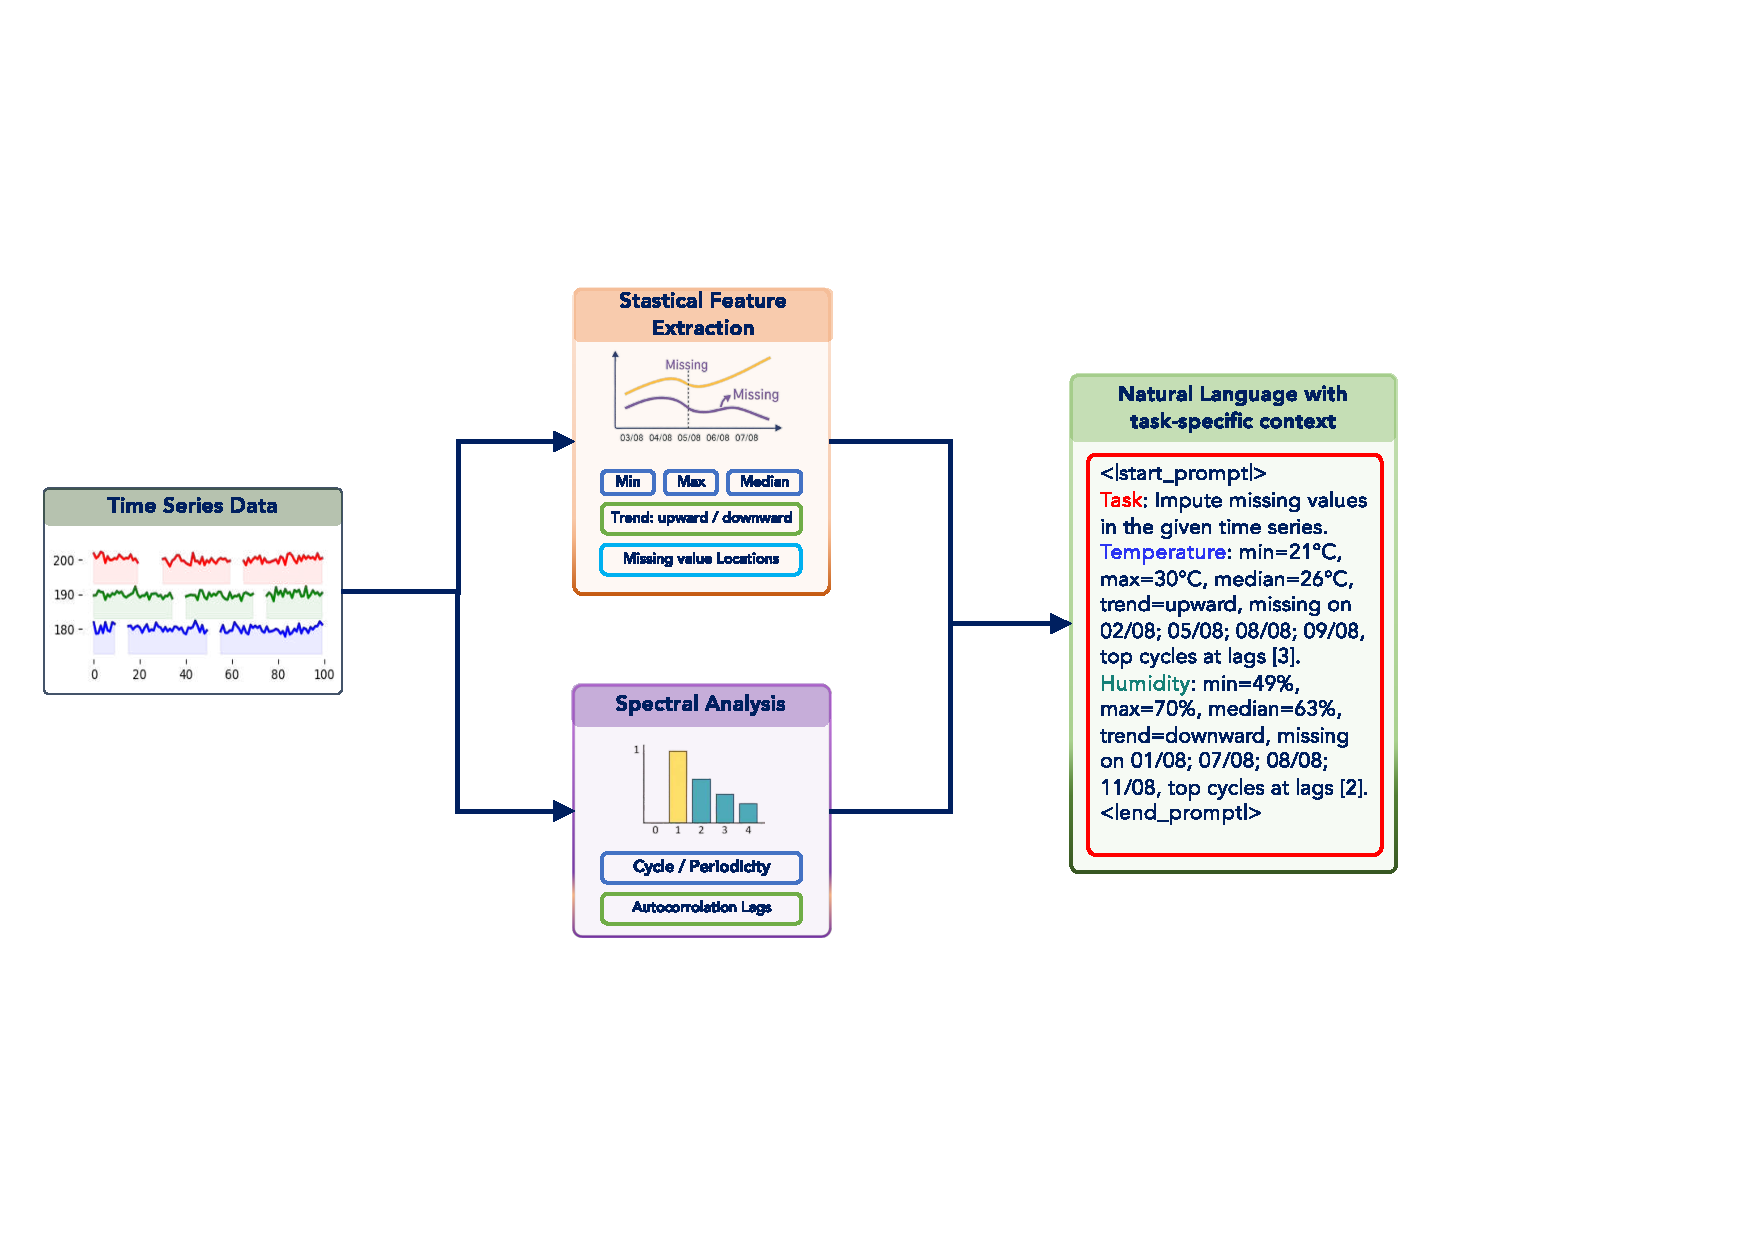
\includegraphics[width=0.8\textwidth]{Prompting.pdf}
    \caption{\small
    Statistical--spectral prompt construction in LLM4Imp.
    From the raw multivariate time series, (i) Statistical Features capture min/max/median, trend, and missing indices;
    (ii) Spectral Analysis detects dominant cycles and autocorrelation lags.
    Both outputs are merged into a natural-language prompt to perform imputation task.}
  \label{fig:prompting_process}
  \vspace{-0.5cm}
\end{figure*}

\section{Introduction}
\label{sec:introduction}
Time-series data are the backbone of modern sensing systems, powering applications from clinical monitoring to
industrial automation and beyond. In real-world deployments, however, missing values are pervasive due to sensor failures,
transmission errors, intermittent connectivity, and irregular sampling. Such gaps can severely degrade the performance of downstream analytics
and decision-making systems.

Traditional statistical imputers, mean filling and last observation carried forward, are simple but fail to capture
temporal dependencies or variable correlations. Deep learning methods have sought to overcome these issues through
various architectural choices. GRU-D \cite{GRU_D,messou2024enhancing} extends gated recurrent units with learnable decay mechanisms to
model temporal gaps explicitly, yet its recurrent design limits long-range dependency capture. BRITS \cite{BRITS}
uses a bidirectional recurrent network with feature-level attention and iterative refinement, improving local accuracy
but incurring high sequential computation cost. Variational autoencoder-based methods such as VAE-Imp \cite{VAE_Impute}
and its variants learn a joint distribution over observed and missing values, enabling probabilistic reconstructions,
yet their latent representations can struggle to encode long-range structure. SAITS \cite{SAITS} employs dual self-attention blocks
to model both temporal and feature dependencies in parallel, but its parameter count and reliance on large training sets
limit scalability. TGAIN \cite{TGAIN} adapts GAN training for imputation by masking observed data and reconstructing
missing entries adversarially, while E2GAN \cite{E2GAN} further explores end-to-end adversarial reconstruction for multivariate sequences;
however, adversarial optimization can be unstable and data-hungry.

Graph-based approaches such as GRIN \cite{GRIN} learn spatial-temporal graphs to propagate information between
related variables, improving accuracy in structured domains but depending heavily on correct graph topology.
NAOMI uses a multi-resolution decoder to fill missing blocks in a coarse-to-fine manner, which reduces
error propagation for short gaps but still accumulates errors over long sequences. MIRACLE integrates
multi-resolution attention with iterative refinement to handle irregular sampling, yet requires multiple passes through
the sequence, increasing latency. BRITS++ improves over BRITS with corruption-aware mechanisms,
while Koopa proposes a unified model for imputation and forecasting, though both approaches remain
computationally expensive. More recently, models such as DeepMVI and MTGNN extend graph
and recurrent paradigms to capture multi-source or cross-sensor evidence for imputation and forecasting.

Transformer-based architectures have become increasingly prominent. Informer and its long-sequence variants
\cite{messou2025tsformer,Reformer,LongNet} reduce quadratic complexity via sparse or scalable attention, but risk losing fine-grained local patterns.
Crossformer \cite{Crossformer} emphasizes cross-dimension dependencies, while TSMixer \cite{TSMixer} demonstrates the
potential of MLP-based alternatives. TimesNet \cite{TimesNetImpute} models temporal variations as 2D structures,
achieving strong forecasting and imputation results but with high computational cost. More recent designs such as TEFN
\cite{TEFN}, TSLANet \cite{Tslanet}, and TimeMixer++ \cite{Timemixerpp} rethink attention and token mixing strategies
to improve efficiency on long-term or dense multivariate series.

Large language models (LLMs) have recently been explored for time-series learning. Time-LLM \cite{TimeLLM} reprograms
frozen LLMs with learnable prompts, enabling forecasting without full fine-tuning. GPT4TS \cite{GPT4TS,messouspec2llm}
extends this paradigm by introducing pre-trained GPT-style models for time-series forecasting. Although promising, these
approaches primarily target forecasting and overlook fine-grained missingness patterns, limiting their applicability to dense imputation tasks.

To address these gaps, we present LLM4IMP, a parameter-efficient framework that reprograms a frozen LLM
(GPT-2 in this experiment) to operate on time-series data without fine-tuning its core parameters.
It leverages the representational power of LLMs while avoiding the computational and data overhead of full fine-tuning. Our main contributions are:
\begin{enumerate}
    \item \textbf{Prompt-Based LLM Reprogramming:} The first imputation framework that reprograms a frozen LLM with natural-language prompts encoding statistical and temporal descriptors of missingness, yielding up to $0.5\%$ error reduction compared with a non-prompted variant.
    \item \textbf{Spectral-Aware Prompt Engineering:} A Fourier-based prompt builder that captures dominant periodic patterns and autocorrelation lags, providing consistent gains of $0.2\%$--$0.3\%$ in absolute error by enriching the LLM context with frequency-domain cues.
    \item \textbf{Patch Embedding for Token Conversion:} A PatchTST-inspired module \cite{PatchTST} that converts multivariate segments into tokenized embeddings, preserving structured temporal information for LLM reasoning.
    \item \textbf{Reprogramming Layer with Cross Attention:} A multi-head cross-attention mechanism that fuses patch and prompt embeddings with residual gating, ensuring effective alignment and improved imputation accuracy.
\end{enumerate}
The remainder of this paper is organized as follows:
Section~\ref{sec:proposed-method} formulates the imputation problem and details the LLM4IMP architecture,
including spectral-aware prompting, patch-based tokenization, and cross-domain reprogramming.
Section~\ref{sec:experiments} describes the experimental setup, including datasets, evaluation metrics, and implementation details,
followed by quantitative and qualitative results.
Finally, Section~\ref{sec:conclusion} summarizes the contributions and outlines potential future research directions.

%% === SECTION II: PROPOSED METHOD ===

\section{Proposed Method}
\label{sec:proposed-method}
\subsection{Problem Formulation}
\label{subsec:problem-formulation}
We consider a multivariate time series
$\mathcal{X} \in \mathbb{R}^{B \times T \times D}$,
where $B$ is the batch size, $T$ the temporal length, and $D$ the number of variables.
A binary mask
$\mathcal{M} \in \{0,1\}^{B \times T \times D}$
indicates the observation pattern, where $\mathcal{M}_{btd} = 1$ denotes an observed value and
$\mathcal{M}_{btd} = 0$ denotes a missing value.
The imputation problem is defined as learning a function
\begin{align}
\hat{\mathcal{X}} = f_{\Theta}\big(\mathcal{X} \odot \mathcal{M},\, \mathcal{M}\big),
\label{eq:imputation_function}
\end{align}
where $f_{\Theta}$ is parameterized by $\Theta$, and $\odot$ denotes element-wise multiplication.
The objective is to reconstruct missing entries $\mathcal{X}_{btd}$ while preserving the observed ones.
Training minimizes the masked mean squared error (MSE) over the missing entries:
\begin{align}
\mathcal{L} =
\frac{\sum\limits_{b=1}^{B} \sum\limits_{t=1}^{T} \sum\limits_{d=1}^{D}
\big(1 - \mathcal{M}_{btd}\big)
\left(\hat{X}_{btd} - X_{btd}\right)^{2}}
{\sum\limits_{b=1}^{B} \sum\limits_{t=1}^{T} \sum\limits_{d=1}^{D}
\big(1 - \mathcal{M}_{btd}\big)}.
\label{eq:loss}
\end{align}
This formulation isolates the loss computation to unobserved entries, ensuring that the model is evaluated solely on its reconstruction capability.
In the following subsections, we describe how LLM4IMP implements $f_{\Theta}$ using a frozen GPT-2 backbone reprogrammed through spectral-aware prompting, patch-based tokenization, and cross-domain attention.

\subsection{Spectral-Aware Prompt Engineering}
\label{subsec:spectral-prompt}

The first stage in LLM4Imp converts the partially observed multivariate time series into a natural-language representation that integrates statistical summaries and spectral characteristics. This stage is designed to bridge the gap between the numerical time-series domain and the token-based semantic space of an LLM. By expressing domain-relevant temporal patterns in a human-readable format, the frozen LLM can reason over the underlying structure without direct parameter updates. The process comprises three steps: missingness representation, feature extraction, and prompt assembly.

\subsubsection{Missingness Representation}
The imputation task begins by identifying the temporal positions of missing observations.
For each sample $b \in \{1, \dots, B\}$, time step $t \in \{1, \dots, T\}$,
and variable $d \in \{1, \dots, D\}$, the missing index set is:
\begin{align}
\mathcal{I}_{bd} = \big\{\, t \ \big|\ \mathcal{M}_{btd} = 0 \big\},
\label{eq:missing-indices}
\end{align}
where $\mathcal{M}_{btd} = 0$ denotes an unobserved entry.
This explicit representation of missingness in~\eqref{eq:missing-indices} serves two purposes:
on one hand, it guides the statistical summarization process to consider only available values;
on the other hand, it encodes positional information directly into the prompt text.

\subsubsection{Statistical Feature Extraction}
\label{subsubsec:stastical-feature-extraction}
The first feature-extraction stream computes descriptive statistics summarizing the distribution and trend of each variable from its observed values.
Given the observed portion of a univariate series $\mathbf{x}_{bd} \in \mathbb{R}^T$, the minimum $\delta_{\min}$, maximum $\delta_{\max}$, and median $\delta_{\mathrm{med}}$ are computed as
\begin{align}
\label{eq:minmax}
\delta_{\min} &= \min_{t:\mathcal{M}_{btd}=1} \mathbf{x}_{bdt}, \quad
\delta_{\max} = \max_{t:\mathcal{M}_{btd}=1} \mathbf{x}_{bdt},
\end{align}
\begin{align}
\label{eq:median}
\delta_{\mathrm{med}} &= \mathrm{med}_{t:\mathcal{M}_{btd}=1}(\mathbf{x}_{bdt}).
\end{align}
The variability of each series is quantified via the standard deviation formulated as follows:
\begin{align}
\sigma_{bd} = \mathrm{std}_{t:\mathcal{M}_{btd}=1}(\mathbf{x}_{bdt}),
\label{eq:std}
\end{align}
which also serves as a relevance score for variable selection in the spectral-analysis stage.
The long-term trend is estimated through least-squares linear regression, with the slope sign $\tau_{bd}$ indicating an upward or downward trajectory:
\begin{align}
\tau_{bd} = \mathrm{sign} \left( \arg\min_{\alpha,\beta} \sum_{t:\mathcal{M}_{btd}=1} \big(\mathbf{x}_{bdt} - \alpha t - \beta\big)^2 \right).
\label{eq:trend}
\end{align}
These descriptors---capturing range \eqref{eq:minmax}, central tendency \eqref{eq:median}, dispersion \eqref{eq:std}, and monotonic behavior \eqref{eq:trend}---form the statistical fingerprint later embedded into the prompt representation.

\subsubsection{Spectral Analysis}
\label{subsubsec:spectral-analysis}
The second feature-extraction stream focuses on identifying periodic and cyclic structures in the time series.
To reduce computational cost and concentrate on informative dynamics, only the $K$ variables with the largest standard deviation $\sigma_{bd}$ from the statistical-analysis stage are processed.
For each selected variable, missing entries are internally replaced with zeros to ensure a complete sequence for frequency-domain processing.
The discrete Fourier transform is then computed as
\begin{align}
\mathcal{F}_{bd}[k] = \sum_{t=0}^{T-1} \mathbf{x}_{bdt} \, e^{-j 2\pi kt / T},
\label{eq:fft}
\end{align}
from which the dominant frequency is obtained as:
\begin{align}
\omega_{bd}^* = \arg\max_{k} \big| \mathcal{F}_{bd}[k] \big|.
\label{eq:frequency}
\end{align}
The corresponding period is calculated as $p_{bd} = T / \omega_{bd}^*$.
In parallel, a time-domain autocorrelation function is evaluated on the observed portion of the signal:
\begin{align}
\rho_{bd}(\ell) = \frac{\sum_{t=1}^{T-\ell} (\mathbf{x}_{bdt} - \bar{x}_{bd}) (\mathbf{x}_{bd,t+\ell} - \bar{x}_{bd})}{\sum_{t=1}^T (\mathbf{x}_{bdt} - \bar{x}_{bd})^2},
\label{eq:lags}
\end{align}
where $\bar{x}_{bd}$ is the mean of the available values.
The $L$ lags $\{\ell_1, \ldots, \ell_L\}$ with the highest $\rho_{bd}(\ell)$ values are retained, capturing the most prominent temporal recurrences.

The statistical descriptors and spectral features obtained from the two extraction streams are subsequently integrated into a unified natural-language prompt, enabling their joint embedding within the LLM space for imputation.

\subsubsection{Prompt Assembly and Embedding}
The outputs of the statistical and spectral streams are merged into a structured natural-language instruction, embedding both numeric summaries and temporal recurrences. A typical prompt form is:
\begin{quote}
\small
\texttt{<|start\_prompt|> Task: Impute missing values for variable $d$. Missing indices: $\mathcal{I}_{bd}$. Min: $\delta_{\min}$, Median: $\delta_{\mathrm{med}}$, Max: $\delta_{\max}$, Trend: $\tau_{bd}$, Dominant period: $p_{bd}$, Top lags: [$\ell_1, \ldots, \ell_L$]. <|end\_prompt|>}
\end{quote}
This representation explicitly encodes the target task, local statistical properties,
and periodic behaviors in a textual format that is semantically interpretable by an LLM.
The prompt is tokenized using the GPT-2 byte-pair encoding (BPE) tokenizer, and the resulting
token IDs are mapped into dense embeddings through GPT-2's frozen embedding layer:
\begin{align}
\mathbf{E}^{\mathrm{prompt}} &= \mathrm{Embed}_{\mathrm{GPT2}}\big(\mathrm{BPE}(\text{Prompt})\big),
\label{eq:prompt-e}
\end{align}
where $\mathbf{E}^{\mathrm{prompt}} \in \mathbb{R}^{B \times D \times L_p \times d_{\mathrm{LLM}}}$,
$L_p$ denotes the token length, and $d_{\mathrm{LLM}}$ is the hidden dimension of the LLM.
These embeddings serve as the semantic context in the subsequent cross-domain attention mechanism,
aligning them with numeric patch representations extracted from the time series.


\subsection{Patch Embedding for Time-Series--to--Token Conversion}
To align the numeric input space with the tokenized LLM space, a PatchTST-inspired embedding module~\cite{PatchTST} is employed.
First, each variable sequence is normalized using reversible instance RevIN as:
\begin{align}
\mathbf{x}'_{bdt} = \frac{\mathbf{x}_{bdt} - \mu_{bd}}{\sigma_{bd} + \epsilon}.
\label{eq:normalization}
\end{align}
Here computed in \eqref{eq:normalization}, $\mu_{bd}$ and $\sigma_{bd}$ are the mean and standard deviation over time for variable $d$ in sample $b$.
The normalized sequence is segmented into overlapping patches of length $P_{\text{size}}$ with stride $P_{\text{stride}}$, producing
$\mathbf{Z} \in \mathbb{R}^{B \times D \times L_{\text{patch}} \times P_{\text{size}}}$.
Each patch is projected to $d_{\text{model}}$ via a linear embedding and positional encoding defined as \(\mathbf{H}^{\text{patch}} \in \mathbb{R}^{B \times D \times L_{\text{patch}} \times d_{\text{model}}}\) :
\begin{align}
\mathbf{H}^{\text{patch}} = \text{PE}\big(\mathbf{Z} \mathbf{W}_p + \mathbf{b}_p\big).
\label{eq:positional-encoding}
\end{align}
This process ensures that the temporal structure of the raw series is preserved while mapping it into a continuous vector space that is compatible with the frozen LLM.

\subsection{Cross-Domain Reprogramming Layer}
The numeric patch embeddings are aligned with semantic LLM embeddings via a multi-head cross-attention layer.
For each variable, patch embeddings serve as \emph{queries} ($Q$) while prompt embeddings provide \emph{keys} ($K$) and \emph{values} ($V$):
\begin{align}
Q &= \mathbf{H}^{\text{patch}} \mathbf{W}^Q, \quad
K = \mathbf{E}^{\text{prompt}} \mathbf{W}^K, \quad
V = \mathbf{E}^{\text{prompt}} \mathbf{W}^V.
\end{align}
Attention is computed using the same principle as proposed by Vaswani et al. \cite{Vaswani2017Attention} for each head $h$ as follow in \eqref{eq:attention}:
\begin{align}
\text{Attn}_h(Q_h, K_h, V_h) &= \text{softmax}\left(\frac{Q_h K_h^\top}{\sqrt{d_k}}\right) V_h.
\label{eq:attention}
\end{align}
Outputs from all heads are concatenated, gated, and combined with residual connections and layer normalization in \eqref{eq:reprog}:
\begin{align}
\mathbf{H}^{\text{reprog}} = \text{LN}\big(\mathbf{H}^{\text{patch}} + \gamma_g \odot \mathbf{O}_{\text{attn}}\big),
\label{eq:reprog}
\end{align}
where $\gamma_g$ is a learnable gating vector.
This stage acts as a cross-domain fusion mechanism, injecting semantic prior knowledge from the prompt into the numeric time-series representation while preserving the original temporal encoding.

\subsection{Output Projection and Reconstruction}
The reprogrammed representations are first processed by the frozen GPT-2 backbone, yielding contextualized token embeddings for each variable and patch position:
\begin{align}
\mathbf{H}^{\text{ctx}} = \mathrm{GPT2}\big(\mathbf{H}^{\text{reprog}}\big),
\label{eq:gpt2_forward}
\end{align}
where $\mathbf{H}^{\text{ctx}} \in \mathbb{R}^{B \times D \times L_{\text{patch}} \times d_{\mathrm{LLM}}}$ contains the semantic-enriched patch representations.
From these, the final patch embedding is selected (the last temporal token per variable in our case) and projected back to the original feature dimension through a linear flatten head defined as:
\begin{align}
\hat{\mathbf{X}}' = \mathbf{H}^{\text{ctx}}_{\text{last}} \mathbf{W}_o + \mathbf{b}_o,
\label{eq:flatten_projection}
\end{align}
where $\mathbf{W}_o \in \mathbb{R}^{d_{\mathrm{LLM}} \times D}$ and $\mathbf{b}_o \in \mathbb{R}^D$ are trainable parameters.
Finally, the inverse RevIN transformation restores each variable to its original scale and distribution:
\begin{align}
\hat{\mathbf{X}} = \mathrm{RevIN}^{-1}\big(\hat{\mathbf{X}}'\big),
\label{eq:revin_inverse}
\end{align}
producing the complete imputed series $\hat{\mathbf{X}} \in \mathbb{R}^{B \times T \times D}$.
This stage concludes the pipeline by transforming enriched contextual embeddings into fully reconstructed time series, ensuring compatibility with the original data domain. The training process is summarized in algorithm~\ref{algo:llm4imp}.

\begin{algorithm}[t]
\caption{Our LLM4Imp Training Pipeline}
\label{algo:llm4imp}
\KwIn{Partially observed series $\mathcal{X} \in \mathbb{R}^{B \times T \times D}$, mask $\mathcal{M}$, patch size $P_{\text{size}}$, patch stride $P_{\text{stride}}$, top-$K$ variables, top-$L$ lags, epochs $E$}
\textbf{Initialize} trainable parameters $\Theta=\{W_p,b_p,W^Q,W^K,W^V,\gamma_g,W_o,b_o\}$;\\
\For{$e=1$ \KwTo $E$}{
  \ForEach{mini-batch $(\mathcal{X},\mathcal{M})$}{
    \textbf{Compute} $\mathcal{I}_{bd} = \big\{\, t \ \big|\ \mathcal{M}_{btd} = 0 \big\}$ via \eqref{eq:missing-indices};
    extract $\delta_{\min},\delta_{\max},\delta_{\mathrm{med}},\sigma_{bd},\tau_{bd}$ via \eqref{eq:minmax}--\eqref{eq:trend}.\\
    \textbf{Compute} $\mathcal{F}_{bd}[k]$ and $\omega_{bd}^*$ via \eqref{eq:fft}--\eqref{eq:frequency};\\
    \textbf{Compute} $\rho_{bd}(\ell) = \frac{\sum_{t=1}^{T-\ell} (\mathbf{x}_{bdt} - \bar{x}_{bd}) (\mathbf{x}_{bd,t+\ell} - \bar{x}_{bd})}{\sum_{t=1}^T (\mathbf{x}_{bdt} - \bar{x}_{bd})^2}$ and keep top-$L$ lags via \eqref{eq:lags}.\\
    \textbf{Build} and embed prompt $\mathbf{E}^{\mathrm{prompt}}$ via \eqref{eq:prompt-e}.\\
    \textbf{Normalize} with RevIN \eqref{eq:normalization};\\
    \textbf{Project} $\mathbf{H}^{\text{patch}}=\mathrm{PE}(\mathbf{Z}W_p+b_p)$ \eqref{eq:positional-encoding}.\\
    \textbf{Apply} attention and fuse $\mathbf{H}^{\text{reprog}}$ via \eqref{eq:attention}--\eqref{eq:reprog}.\\
    \textbf{Forward} frozen GPT-2; flatten/project; inverse RevIN via \eqref{eq:gpt2_forward}--\eqref{eq:revin_inverse} $\to \hat{\mathcal{X}}$.\\
    \textbf{Compute} $\mathcal{L}$ via \eqref{eq:loss}; backpropagate $\nabla_{\Theta}\mathcal{L}$; update $\Theta$ with optimizer.
  }
}
\KwOut{Imputed series $\hat{\mathcal{X}}$}
\end{algorithm}

%% === SECTION III: EXPERIMENTS ===

\section{Experiments}
\label{sec:experiments}

\subsection{Implementation Details}
\label{subsec:implementation}
LLM4Imp is evaluated against five baselines: SAITS, TSLANet, TEFN, and TimeMixer++ provided by PyPOTS \cite{PyPOTS}. Experiments are conducted on four publicly available multivariate time-series datasets: PhysioNet2012, Beijing Multisite Air Quality, Italy Air Quality, and Solar Alabama. Each dataset is divided into 70\% training, 15\% validation, and 15\% testing. For LLM4Imp, missing rates of $0.1, 0.2, 0.3, 0.4$, and $0.5$ are tested with a fixed batch size of 32, embedding dimension $d_{\mathrm{model}}$ of 64, attention heads of 6, and 1 layers. All implementations use PyTorch $2.5$ with Python $3.10$ on Ubuntu 24.04, running on a server equipped with dual AMD EPYC 7302 16-Core processors ($32$ physical cores, $2$ NUMA nodes, $3.0$~GHz base, $3.3$~GHz boost). The GPT-2 backbone remains frozen. Performance is measured using mean absolute error (MAE), mean squared error (MSE) for, root mean squared error (RMSE), and mean relative error (MRE) over the prediction horizon and all variables, optimized with AdamW for $10$ epochs and an input length of $96$.
\begin{table*}[!ht]
\centering
\caption{Imputation results on four benchmarks across missing rates from MR from $0.1$ to $0.5$. Metrics MAE and MSE, where the lower the better. The best result in each column is highlighted in \textbf{bold}, and the second best is \underline{underlined}.}
\label{tab:main-results}
\begin{tabular}{lcccccccccc}
\toprule
& \multicolumn{2}{c}{MR=0.1} & \multicolumn{2}{c}{MR=0.2} & \multicolumn{2}{c}{MR=0.3} & \multicolumn{2}{c}{MR=0.4} & \multicolumn{2}{c}{MR=0.5} \\
\cmidrule(lr){2-3}\cmidrule(lr){4-5}\cmidrule(lr){6-7}\cmidrule(lr){8-9}\cmidrule(lr){10-11}
Dataset / Model & MAE $\downarrow$ & MSE $\downarrow$ & MAE $\downarrow$ & MSE $\downarrow$ & MAE $\downarrow$ & MSE $\downarrow$ & MAE $\downarrow$ & MSE $\downarrow$ & MAE $\downarrow$ & MSE $\downarrow$ \\
\midrule
\multicolumn{11}{c}{\textbf{PhysioNet2012}}\\
SAITS        & 0.438 & 0.511 & 0.451 & 0.550 & 0.467 & 0.554 & 0.488 & 0.586 & 0.518 & 0.642 \\
TEFN         & 0.515 & 0.739 & 0.541 & 0.810 & 0.566 & 0.835 & 0.594 & 0.885 & 0.625 & 0.962 \\
TSLANet      & 0.714 & 1.029 & 0.710 & 1.034 & 0.709 & 1.013 & 0.707 & 1.015 & 0.707 & 1.031 \\
TimeMixer++  & 0.429 & \textbf{0.471} & 0.428 & \textbf{0.499} & \textbf{0.432} & \textbf{0.502} & \textbf{0.435} & 0.526 & 0.445 & 0.552 \\
LLM4Imp      & \textbf{0.411} & 0.511 & \textbf{0.426} & 0.553 & 0.442 & 0.563 & 0.461 & \textbf{0.501} & \textbf{0.432} & \textbf{0.550} \\
\midrule
\multicolumn{11}{c}{\textbf{Beijing Multisite Air Quality}}\\
SAITS        & \textbf{0.254} & \textbf{0.339} & \textbf{0.261} & \textbf{0.383} & \textbf{0.265} & \textbf{0.361} & \textbf{0.272} & \textbf{0.364} & \textbf{0.286} & \textbf{0.371} \\
TEFN         & 1.273 & 3.266 & 1.277 & 3.274 & 1.284 & 3.279 & 1.295 & 3.315 & 1.302 & 3.330 \\
TSLANet      & 0.761 & 1.165 & 0.761 & 1.203 & 0.758 & 1.169 & 0.757 & 1.160 & 0.757 & 1.152 \\
TimeMixer++  & \underline{0.392} & 0.496 & \underline{0.413} & 0.576 & \underline{0.430} & \underline{0.546} & 0.495 & 0.606 & 0.588 & 0.706 \\
LLM4Imp      & 0.395 & \underline{0.495} & 0.419 & \underline{0.549} & 0.449 & 0.557 & \underline{0.483} & \underline{0.594} & \underline{0.524} & \underline{0.647} \\
\midrule
\multicolumn{11}{c}{\textbf{Italy Air Quality}}\\
SAITS        & 0.551 & 1.026 & 0.565 & 1.079 & \underline{0.573} & 1.126 & \underline{0.581} & 1.125 & \underline{0.589} & 1.148 \\
TEFN         & 2.103 & 7.765 & 2.166 & 8.120 & 2.193 & 8.257 & 2.243 & 8.607 & 2.262 & 8.779 \\
TSLANet      & 0.805 & 1.594 & 0.810 & 1.660 & 0.817 & 1.704 & 0.802 & 1.633 & 0.799 & 1.597 \\
TimeMixer++  & \textbf{0.320} & \textbf{0.356} & \textbf{0.403} & \underline{0.554} & 0.667 & \underline{0.707} & 0.680 & \underline{0.738} & 0.732 & \underline{0.833} \\
LLM4Imp      & \underline{0.431} & \underline{0.455} & \underline{0.466} & \textbf{0.518} & \textbf{0.517} & \textbf{0.658} & \textbf{0.530} & \textbf{0.666} & \textbf{0.558} & \textbf{0.731} \\
\midrule
\multicolumn{11}{c}{\textbf{Solar Alabama}}\\
SAITS        & \textbf{0.128} & \textbf{0.064} & \textbf{0.130} & \textbf{0.066} & \textbf{0.120} & \textbf{0.065} & \textbf{0.121} & \textbf{0.064} & \textbf{0.122} & \textbf{0.065} \\
TEFN         & 1.484 & 4.225 & 1.499 & 4.297 & 1.501 & 4.309 & 1.500 & 4.303 & 1.501 & 4.303 \\
TSLANet      & 0.783 & 0.831 & 0.781 & 0.831 & 0.780 & 0.826 & 0.777 & 0.818 & 0.775 & 0.810 \\
TimeMixer++  & \underline{0.452} & \underline{0.348} & \underline{0.465} & \underline{0.420} & \underline{0.492} & \underline{0.518} & \underline{0.543} & \underline{0.476} & \underline{0.541} & \underline{0.467} \\
LLM4Imp      & 0.568 & 0.579 & 0.588 & 0.584 & 0.609 & 0.590 & 0.630 & 0.600 & 0.650 & 0.610 \\
\bottomrule
\end{tabular}
\end{table*}
\subsection{Parameter Efficiency}
Parameter efficiency is a key consideration for large-scale time-series imputation.
Table~\ref{tab:params} summarizes the total number of parameters, the subset updated during training, and their ratio across all evaluated models.
Classical architectures such as SAITS, TEFN, and TSLANet optimize all parameters, while TimeMixer++ also requires updating nearly all weights.
In contrast, LLM4Imp reprograms a frozen GPT-2 backbone and restricts training to less than $9\%$ of the parameters, achieving a substantial reduction in training cost.
This parameter efficiency highlights the scalability of the proposed approach, while the performance results in Table~\ref{tab:main-results} confirm that accuracy is preserved despite the smaller trainable footprint.

\begin{table}[!ht]
\centering
\caption{Comparison of model parameter usage.}
\label{tab:params}
\begin{tabular}{lrrr}
\toprule
Model & Total Params & Trainable Params & Trainable (\%) \\
\midrule
SAITS        & 79,792        & 79,792        & 100 \\
TEFN         & 36,420        & 36,420        & 100 \\
TSLANet      & 584,674       & 584,674       & 100 \\
TimeMixer++  & 613,635       & 608,771       & 99.2 \\
LLM4Imp (GPT2) & 128,520,192   & 11,168,256    & \textbf{8.7} \\
\bottomrule
\end{tabular}
\vspace{-0.5cm}
\end{table}

\subsection{Main Results}
\label{subsec:main-results}
Table~\ref{tab:main-results} reports the imputation results across four benchmarks under missing rates from $0.1$ to $0.5$, with MAE and MSE as evaluation metrics. Several observations can be drawn.

First, the performance of SAITS demonstrates that lightweight attention-based architectures remain highly competitive on low-dimensional datasets. In particular, SAITS achieves the lowest errors on Solar Alabama, which has relatively simple seasonal patterns. However, the gap between MAE and MSE values for SAITS on this dataset suggests sensitivity to extreme deviations, indicating limited robustness in the presence of outliers.
Second, TimeMixer++ shows improvements on more complex datasets such as PhysioNet2012 and Italy Air Quality, benefiting from its ability to leverage pretrained components. Nevertheless, its performance is inconsistent as the missing rate increases, with errors rising more sharply than those of LLM4Imp. This instability highlights the difficulty of maintaining generalization when higher proportions of data are absent.
Third, LLM4Imp demonstrates stable and robust behavior across all datasets, becoming particularly strong on higher-dimensional or irregular datasets such as PhysioNet2012 and Beijing Multisite Air Quality. Unlike SAITS and TimeMixer++, which degrade more noticeably at missing rates of $0.4$ and $0.5$, LLM4Imp consistently maintains lower errors. This robustness confirms the effectiveness of the statistical--spectral prompt mechanism and cross-domain reprogramming in preserving temporal information under severe missingness.
Finally, these accuracy trends correlate with the parameter efficiency analysis in Table~\ref{tab:params}. While SAITS and TEFN achieve efficiency by virtue of their smaller architectures, they fail to generalize to more complex datasets. Conversely, TimeMixer++ improves accuracy but requires training nearly all of its parameters. LLM4Imp strikes a favorable balance: despite updating less than $9\%$ of its parameters, it delivers the best or second-best performance in nearly all scenarios. This balance between accuracy and efficiency demonstrates the practical advantage of reprogramming a frozen LLM rather than relying on full fine-tuning architecture.

\subsection{Ablation Study}
An ablation study is conducted on two complementary datasets: Beijing Multisite Air Quality, characterized by correlated spatial--temporal dynamics, and PhysioNet2012, which contains heterogeneous clinical signals. The missing rate is fixed at $0.3$, with the model configured to one layer, six attention heads, $d_{\mathrm{model}}=64$, and $d_{\mathrm{ffn}}=128$. Three variants are evaluated: the complete model with both prompt and reprogramming modules, a version with prompts only, and a version with reprogramming only. The trivial case disabling both modules is excluded since it prevents meaningful alignment between time-series patches and prompts.

Table~\ref{tab:ablation} reports MAE, MSE, RMSE, and MRE. On Beijing Multisite Air Quality, removing the prompt increases MAE by $+0.0017$ and RMSE by $+0.0031$, while discarding the reprogramming layer results in smaller increases ($+0.0002$ MAE and $+0.0012$ RMSE). On PhysioNet2012, the effect is stronger: eliminating the prompt raises MAE by $+0.0027$ and RMSE by $+0.0031$, whereas disabling reprogramming causes $+0.0012$ MAE and $+0.0005$ RMSE. In both datasets, the MSE and MRE metrics follow the same trend, with the prompt contributing more noticeable improvements on PhysioNet2012 and reprogramming showing a consistent but smaller benefit.
Overall, the results demonstrate that each module provides complementary advantages: the reprogramming layer ensures alignment between patch and prompt embeddings, while the prompt mechanism enriches the model with semantic guidance. Their combination consistently yields the best performance, confirming that both are critical for effective imputation.

\begin{table*}[!ht]
\centering
\caption{Ablation on Beijing Multisite Air Quality and PhysioNet2012 at missing rate $0.3$. Metrics are mean absolute error (MAE), mean squared error (MSE), root mean squared error (RMSE), and mean relative error (MRE).}
\label{tab:ablation}
\begin{tabular}{lcccccccc}
\toprule
\multirow{2}{*}{Configuration} & \multicolumn{4}{c}{Beijing Multisite Air Quality} & \multicolumn{4}{c}{PhysioNet2012} \\
\cmidrule(lr){2-5}\cmidrule(lr){6-9}
 & MAE $\downarrow$ & MSE $\downarrow$ & RMSE $\downarrow$ & MRE $\downarrow$ & MAE $\downarrow$ & MSE $\downarrow$ & RMSE $\downarrow$ & MRE $\downarrow$ \\
\midrule
Full model (Prompt + Reprog) & \textbf{0.4490} & \textbf{0.5570} & \textbf{0.7463} & \textbf{0.5966} & \textbf{0.5429} & \textbf{0.6630} & \textbf{0.8143} & \textbf{0.7682} \\
Prompt only                   & 0.4507 & 0.5616 & 0.7494 & 0.5988 & 0.5456 & 0.6691 & 0.8174 & 0.7718 \\
Reprogramming only            & 0.4492 & 0.5588 & 0.7475 & 0.5969 & 0.5441 & 0.6650 & 0.8148 & 0.7695 \\
\bottomrule
\end{tabular}
\end{table*}

%% === SECTION IV: CONCLUSION ===

\section{Conclusion}
\label{sec:conclusion}
We have presented \textbf{LLM4IMP}, a parameter-efficient framework that reprograms a frozen GPT-2 for dense, multivariate time-series imputation. By integrating spectral prompt engineering, PatchTST-inspired tokenization, and a cross-domain reprogramming layer, LLM4IMP leverages both semantic reasoning and temporal structure without the cost of full model fine-tuning.
Our experiments on four benchmarks datasets demonstrate that LLM4IMP achieves marginal reconstruction accuracy compared to state-of-the-art algorithms.
Future work can explore extending this framework to irregularly sampled sequences and multimodal data fusion settings to further broaden its applicability in real-world sensing systems.

\bibliographystyle{IEEEtran}
\bibliography{IEEEtran}

\end{document}
